
In order to convert from strip number to 2$\theta$-angle, an accurate angular calibration of the detector must be performed (for details see the paper Bergamaschi, A. et al. (2010). J. Synchrotron Rad. 17, 653-668). \\

For this purpose, a series of patterns of a powder standard with symmetric peaks (e.g. silicon) must acquired while shifting the detector by an angular step of the order of about 2\% of the module size. During the measurement, a strong intensity peak (e.g. Si(111)) should pass through the field of view of every module such that it can be used as a reference angular position to perform the calibration of the modules position.\\

In a first step, the   peak is fitted with a Gaussian in order to determine its position $C_{peak}$ in channel number for each of the acquired patterns.\\
In a second step, for each module $i$, the encoder position  $\Theta_e$  is fitted as a function of the peak position  $C_{peak}$  according to:
\begin{equation}\label{eq:angcal}
\Theta_e=\Theta_o^i-\arctan\Big(\frac{p \cdot (C_{peak}-C_{center}^i)}{R^i}\Big),
\end{equation} 
where the parameters $\Theta_o^i$ is the angular offset with respect to the diffractometer zero position, $C_{center}^{i}$ is the central channel  and $R^i$ is the distance of the module $i$ from the diffractometer center while $p=50~\mu m$ is the strip pitch of the detector. \\
Finally, the global offset of the detector system is precisely determined by refining a silicon pattern at a well-defined energy (i.e., knowing the position of the peak).

The same function of equation~\ref{eq:angcal}, with the parameters obtained from the calibration, is used in order to convert from channel number to 2$\theta$-angle.

The parallax at the borders of the modules due to the thickness of the silicon sensor is a function of the X-ray energy (higher energy X-rays are absorbed deeper inside the sensor) and is of the order of 0.2~mdeg at 12~keV and 0.5~mdeg at 30~keV. \\
The differences in pixel size due to the different portion of solid angle covered by the strips on the border of the modules and  the higher efficiency due to the longer path of the X-rays in the sensor are removed by the flat field correction. This also normalizes additional differences in pixel size between channels which are also present because of mismatches in the strip sensor fabrication and in fluctuations of the channels threshold level.
 
Patterns acquired at different detector positions are generally merged together  in order to fill the gaps between the modules and correct possibly bad functioning channels. In this procedure the data from different positions which are closer than 4~mdeg (the average pixel size) are averaged and the new position is set to the mean of the positions of the original points.


The position and width of the peaks results from a fit over several detector channels. Geometrical distortions might disturb this determination mainly because of errors in the angular calibration, fluctuations in the encoder position, variations between channels and parallax effects.\\
The resolution in locating the peak center and determining its width and integrated intensity has been estimated by acquiring several patterns of a LaB$_6$ sample in a 300~$\mu$m capillary with the detector shifted in 5~mdeg steps between 30.4 and 36.5 degrees. The 16~peaks acquired have been fitted with a Gaussian function plus background and the fluctuations on the fitted parameters have been calculated. The resulting average resolutions are  0.63$\pm$0.06~mdeg for the peak center and 0.22$\pm$0.05~mdeg for the peak Full-Width at Half-Maximum (FWHM) for an average peak FWHM of 27.0$\pm$2.5~mdeg. \\
These results show that  the angular calibration allows a resolution in determining the peaks position and width which is appropriate for structural determination.

\section{Data acquisition}

The angular calibration consists in acquiring a set of diffraction patterns of a well known powder standard (e.g. Silicon) at different encoder positions.  In order to facilitate the procedure, the sample should not emit fluorescent light and should present relatively symmetric peaks. \\
During the measurement, a strong intensity peak (e.g. Si(111)) should pass through the field of view of every module such that it can be used as a reference angular position to perform the calibration of the modules position. In general the highest peak will be used for the calibration, but this is not necessary in case there would be e.g. geometrical limitations for shifting the detector. \\ \textbf{Do not forget to properly position the beam stopper if the detector is scanned in front of the direct beam.}\\
The detector should be shifted of an angular step of the order of about 2\% of the module size, such that about 50 patterns can contribute to the fitting of the 3 parameters necessary for the angular calibration.\\
 
All the angular calibration procedure should be acquired using a trimmed detector with the threshold set at half of the X-ray energy (Assuming no fluorescent element in the standard). A flat field should also be acquired in order to precisely correct the data, while the X-ray intensity should be kept lower than about 100~kHz per strip in order to avoid the need for rate corrections.

A rough angular conversion file starting from a previous calibration or from the geometric characteristics of the mechanics is an advantage. The angular conversion file should contain a line for each module of the detector with its module number $i$, center  $C_{center}^{i}$ and error, conversion radius $p/R^i$ and error, offset $\Theta_o^i$ and error:
\begin{verbatim}
module 0 center 639.5 +- 0 conversion 6.56E-05 +- 0 offset 0 +- 0
\end{verbatim}
Also the \textit{global offset} value of the beamline should be approximately known i.e. the angular position of channel 0 of module 0 when the motor is set at 0. \\
All the documentation assumes that the detector is oriented in the same direction as the encoder position i.e. large channel number at higher angles (both per module and absolute). If this is not the case, the \textit{angular direction} should be set to -1. 

\subsection{Software}

For the acquisition ot the data you need to install the slsDetector software package (please refere to separate documentation). The use of the GUI is optional and all operations can be performed also using the text client.\\

Please make sure that you have edited the \\
\textit{slsDetectorSoftware/usersFunctions/angleFunction.h} \\
in order to match the angular conversion for your geometry and \\
\textit{slsDetectorSoftware/usersFunctions/usersFunctions.cpp} \\
in order to be able to move the detector and read out its position by using the slsDetector software.

In the following the command to acquire a dataset for the angular calibration with an exposure time of 1~s, and position shift 
\begin{verbatim}
#setup angular calibration log mode
> sls_detector_put angcallog 1 
#set exposure time to 1s
> sls_detector_put exptime 1. 
#setup threshold scan
> sls_detector_put scan0script position 
#setup the precision for the scan variable in the file name
> sls_detector_put scan0prec 2 
#set scan range between 20deg and -60deg, step of -0.1deg
# (at 12.4 keV the Si(111) peak is at approx 19deg
> sls_detector_put scan0range 20 -60 -0.1 
#acquire the data
> sls_detector_acquire
#unset angular calibration log mode
> sls_detector_put angcallog 0
\end{verbatim}

With the GUI you can obtain the same results by clicking on the \textit{Angular calibration} log button in the advanced tab (see figure~\ref{fig:guiangcallog}) and setting up the motor position scan in the Actions tab (see figure~\ref{fig:guiposscan}). The exposure time should also be set in the measurement tab.



Additional to the data files, the acquisition will produce a .angcal file containing an header and, for each step of the acquisition, the exect value of the motor position and the file name. \\
In case you forgot to enable the angcallog flag in the software, you can produce the file with the syntax as follows, assuming that you know the exact values of your encoder for each frame:
\begin{verbatim}
type Mythen
maxmod 32
nmod 32
angconv /scratch/angcal20120422/ang.off
globaloff 5.088
fineoff 0.0
angdir 1
ffdir /scratch/angcal20120422/
flatfield flatfield_E12keV_T6keV_0.raw
badchannels /scratch/cal/bad.chans
19.99998 angcal_S20.00_0
19.90001 angcal_S19.90_0
19.79999 angcal_S19.80_0
19.70002 angcal_S19.70_0
......
\end{verbatim}



\begin{figure}
\caption{Acquisition GUI window to enable the angular calibration log.} \label{fig:guiangcallog}
\includegraphics[width=\textwidth]{enable_angcal.eps}
\end{figure} 

\begin{figure}
\caption{Acquisition GUI window to setup the motor position scan.} \label{fig:guiposscan}
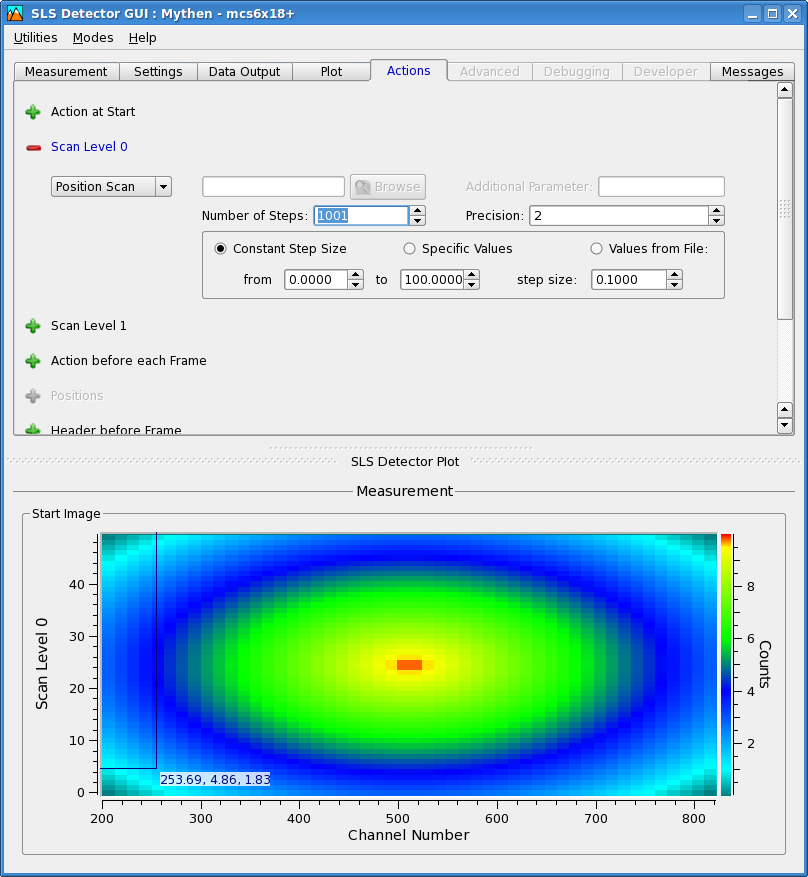
\includegraphics[width=\textwidth]{position_scan.eps}
\end{figure} 
\newpage

\section{Data analysis}

The data analysis consists in fitting with a gaussian the selected peak of the powder pattern for each position in order to determine its position is channel number as a function of the encoder position. \\
In a second step, for each module, the channel vs. encoder curve is fitted in order to extrapolate the three parameters necessary for the angular conversion and the result is written to file

\subsection{Software}

The software used for the angular calibration data analysis is based on root (see http://root.cern.ch).\\
This can be downloaded as binary or installed from sources. The version of the software should not play an important role, but up to now everything has been implemented and tested using version 5.20.

To start the data analysis simply launch:
\begin{verbatim}
> ./angularCalibrationWizard 
\end{verbatim}

\begin{figure}
\caption{Overview of the nagular calibration dataset.} \label{fig:setangcal}
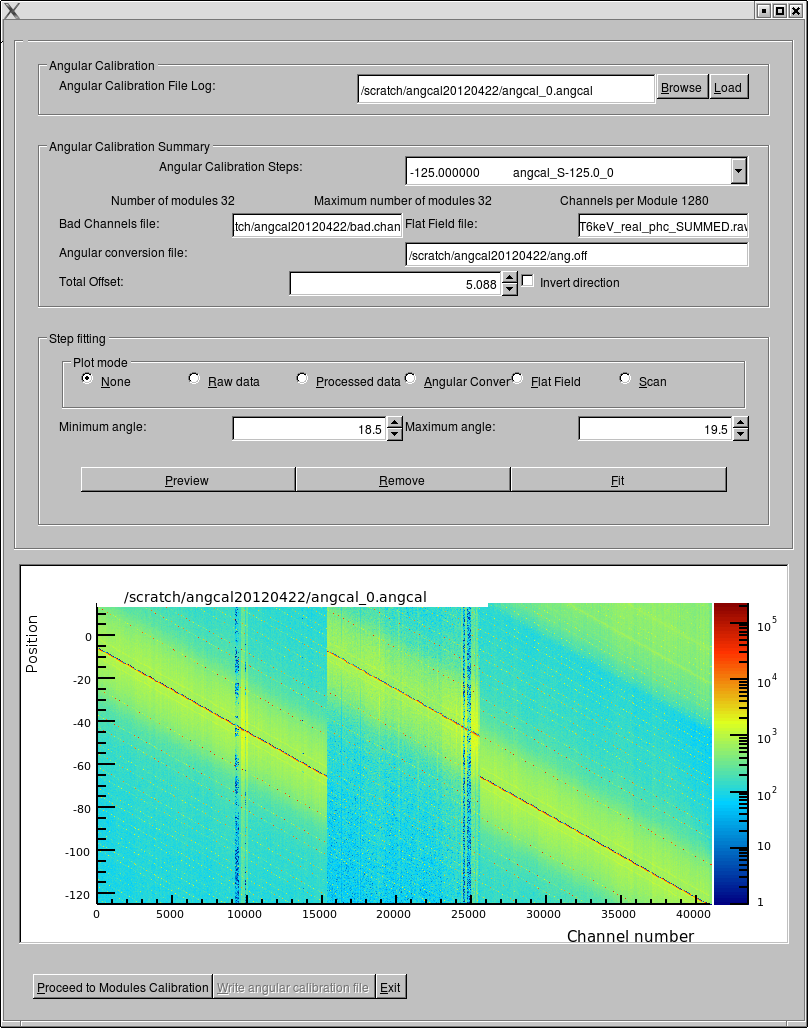
\includegraphics[width=\textwidth]{setupAngcal.eps}
\end{figure} 

To setup the angular calibration dataset, the .angcal file should be selected (or digited) and the load button should be pressed to confirm. The parameters of the angular calibration are then read to the file and the data loaded for a quick overview (see figure~\ref{fig:setangcal}).\\
The software assumes that the data files (.raw) and the .encal file are in the same directory.\\
A 2D color plot will show a rebinned overview of the dataset. The peak to be fitted should be visible as a high intensity diagonal line passing through all the channels.


\begin{figure}
\caption{Preview of the fitting of the Si(111) peak for one of the detector positions.} \label{fig:peakfit}
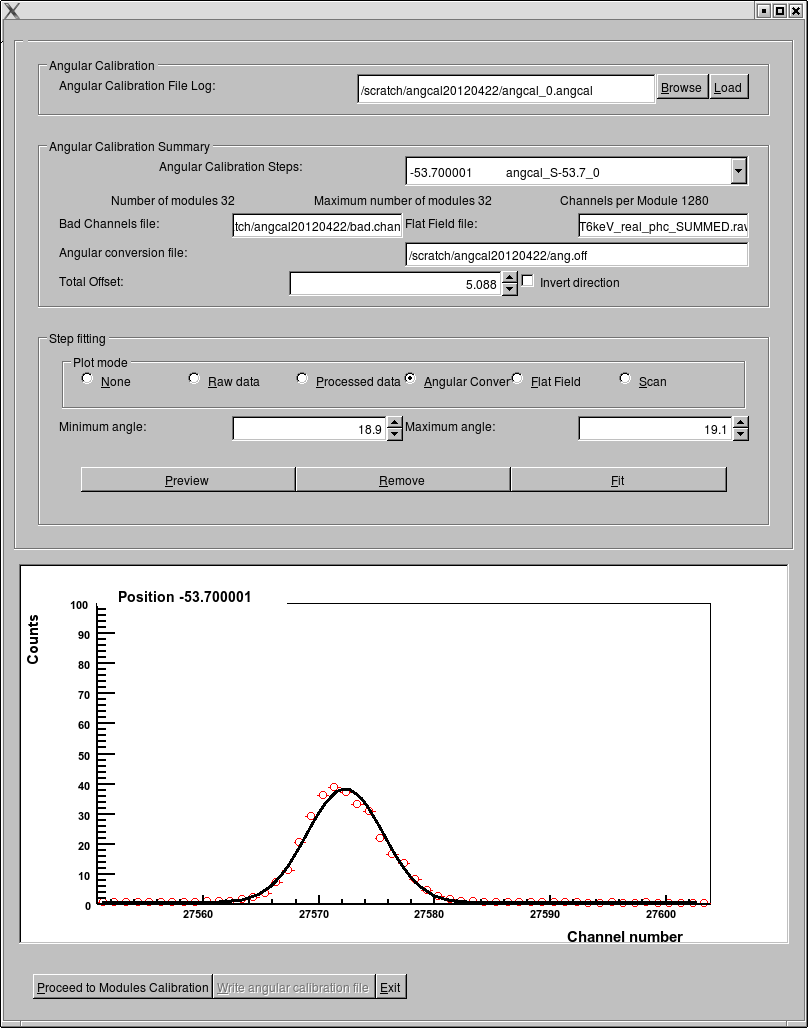
\includegraphics[width=\textwidth]{peakFit.eps}
\end{figure} 

For a more detailed view of the data, one can select an angular calibration step from the combo box, select the plot mode (raw data or processed data as a function of channel number, processed angular converted data, flat field data, or again an overview of the whole dataset). \\
By (right) clicking close to the axis you are able to zoom in/out, set the scale to logarithmic etc.\\

If the bad channel list, angular conversion file or flat field file are changed compared to the acquisition, they can be reloaded by editing the correspondent text entries and pressing enter.

In particular, the angular converted data should be checked in order to view the position of the selected peak. In this case, the plot will be zoomed to the angular region slected in the minimum and maximum angle entries. By pressing fit, the fit of the peak in the selected angular range will be shown (see figure~\ref{fig:peakfit}).  It is useful to check that it works properly in several positions such that then the sequential fitting on all steps can give good results.

To automatically fit all positions simply press \textit{Proceed to Modules Calibration} and wait until all steps are fitted. This can take sometime, depending on the number of steps.


\begin{figure}
\caption{Window for fitting the angular calibration parameters of a module.} \label{fig:anglefit}
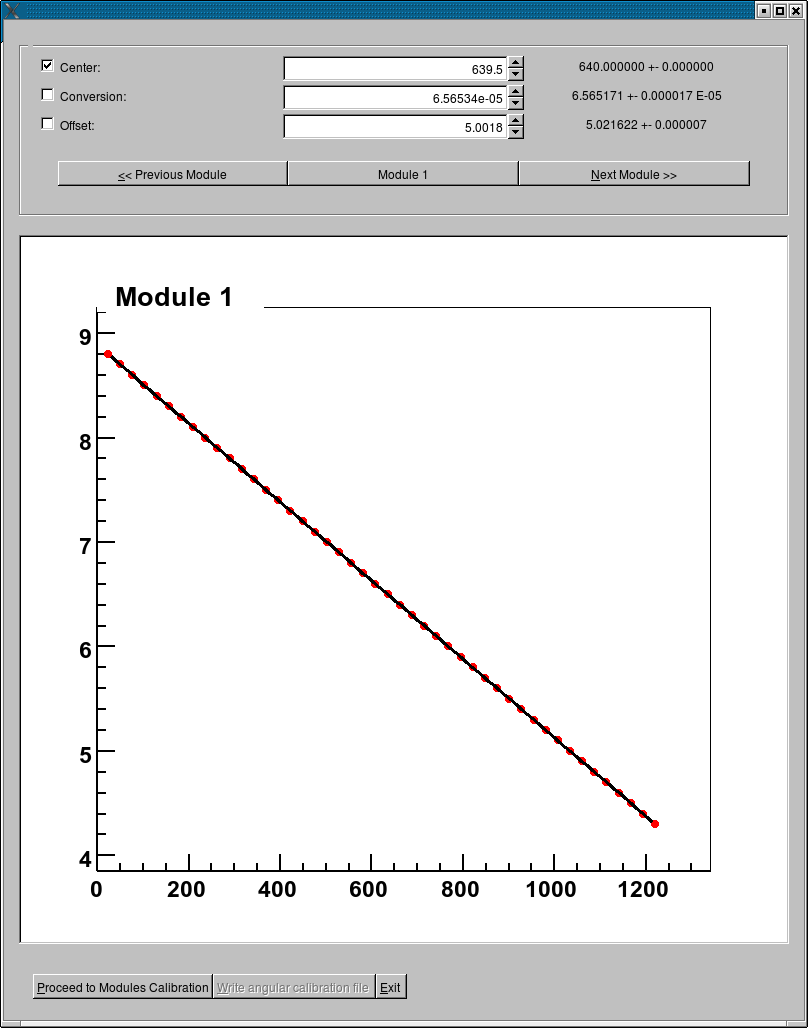
\includegraphics[width=\textwidth]{angleFit.eps}
\end{figure} 





In the module calibration window (see figure~\ref{fig:anglefit}), you will be able to fit the channel number to encoder position curve to estimate the three angular calibration parameters for each module.\\
The entries show the angular calibration parameters used for approximate angular conversion in the previous step of the calibration. These can be edited and will be used as start parameters for the fit.
By clicking on the check box next to the parameters, the selected parameter will be set and fixed during the fit. Often the center is used as a fix parameter.\\
It is possible to navigate between modules by using the Previous and Next module buttons. To refit the current module (e.g. after changing one of the parameters) simply re-click on the module number.

After fitting all modules you can click on the \textit{Write Angular Calibration} button, select the file name to write to and save the calibration angulat calibration data. Please note that the offset of module 0 will always be 0 and the other values will be rescaled to its value. Therefore the global offset of the steup will always need to be specified for a proper angular conversion unless the home of the encoder will not be redifined.

\section{Setup calibration files}

To use the generated angular calibration files, using the text client:
\begin{verbatim}
sls_detector_put angconv /scratch/ang_new.off 
\end{verbatim}
while for the GUI the file name should be specified in the configuration file (works also for the text client).
\end{document}

